\section{Introduction}\label{sec:intro}

\begin{figure}[b]
    \centering
    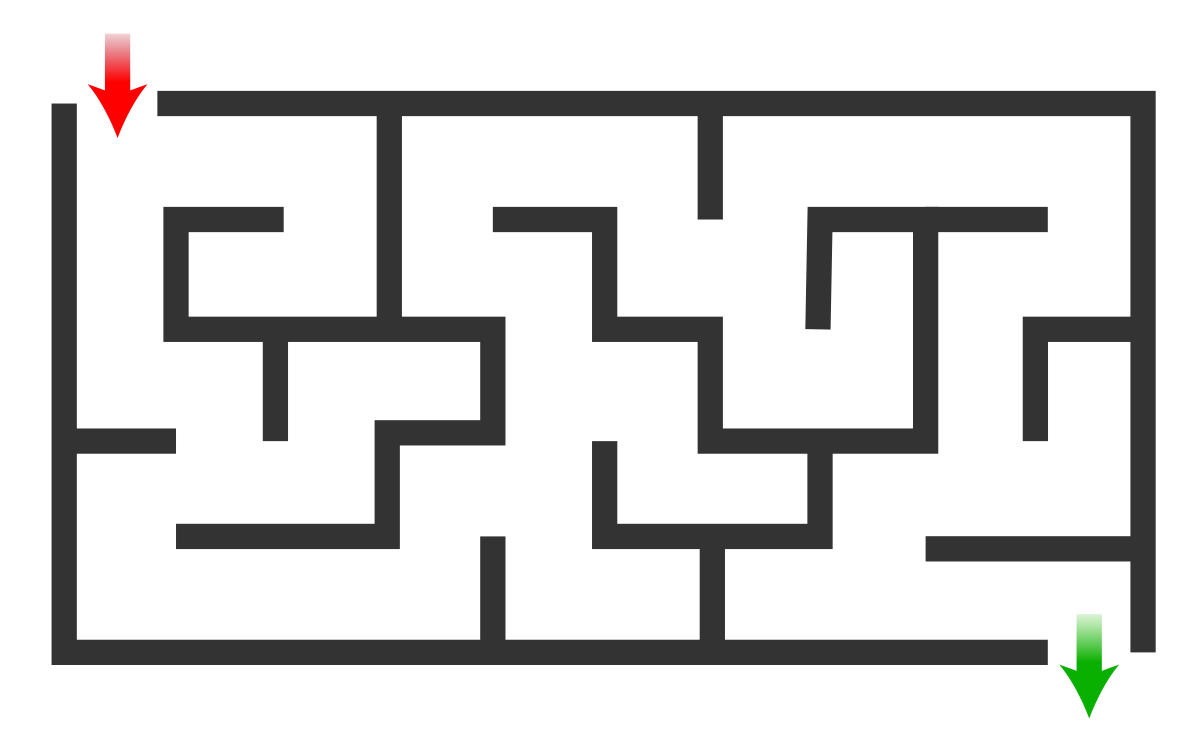
\includegraphics[scale=0.1]{img/Maze_simple.svg.png}
    \caption{Example of a Maze}\label{fig:fig1}
\end{figure}

The main objective of this project is to use different Inductive Logic Programming (ILP) techniques on the same problem in order to highlight
their differences. Despite the importance of performance differences (see Section~\ref{sec:perf}), we are also going to focus on the differences
concerning the approach to the problem, as some of us had to take completely different paths in order to reach similar goals.\\

Our work is focussed on the Maze problem. This problem consists in finding a path from point \texttt{A}
to point \texttt{B} in a labirinth-like shaped map (see Figure~\ref{fig:fig1}). A variety of classical algorithms
can be used to solve this problem, starting from the most naïve wall following algorithm to more complex and elaborated
ones exploiting graph theory concepts.\\
By approaching this simple problem with ILP though, it is possible to extend it into a much more sophisticated and interesting
problem. For instance, it allowed us to start with the assumption that the problem's main character (the
one we shall refer to as \emph{agent}) has no knowledge about \emph{how} to move. Consequently, before even trying
to solve the Maze, the agent needs to \emph{learn} what a \emph{move} is and, more specifically, what a \emph{legal} move is. The second
step consisted into \emph{teaching} the agent how to reach two distant cells. Lastly, in order to solve the Maze, it is either possible
to keep using ILP in order to find a solution or use the learned rules in order to implement them in a logic programming model of the planning
problem.\\